\documentclass{article}
\usepackage[utf8]{inputenc}
\usepackage{listings}
\usepackage{color}
\usepackage[italian]{babel}
\usepackage{graphicx,wrapfig,lipsum}
\usepackage{float}
\usepackage{amsmath}
\usepackage{hyperref}
\usepackage{graphicx}
\usepackage{subcaption}
\definecolor{dkgreen}{rgb}{0,0.6,0}
\definecolor{gray}{rgb}{0.5,0.5,0.5}
\definecolor{mauve}{rgb}{0.58,0,0.82}
\usepackage{listings}
\usepackage{xcolor}
\usepackage{booktabs}
\usepackage{changepage} % Per modificare la larghezza della pagina
\definecolor{codegreen}{rgb}{0,0.6,0}
\definecolor{codegray}{rgb}{0.5,0.5,0.5}
\definecolor{codepurple}{rgb}{0.58,0,0.82}
\definecolor{backcolour}{rgb}{0.95,0.95,0.92}

\lstdefinestyle{mystyle}{
    backgroundcolor=\color{backcolour},   
    commentstyle=\color{codegreen},
    keywordstyle=\color{magenta},
    numberstyle=\tiny\color{codegray},
    stringstyle=\color{codepurple},
    basicstyle=\ttfamily\footnotesize,
    breakatwhitespace=false,         
    breaklines=true,                 
    captionpos=b,                    
    keepspaces=true,                 
    numbers=left,                    
    numbersep=5pt,                  
    showspaces=false,                
    showstringspaces=false,
    showtabs=false,                  
    tabsize=2
}
\lstset{style=mystyle}


\title{Report Progetto Intelligenza Artificiale}
\author{Gabriele Genovese 0001136707\\ Erik Koci 0001136721 }

\begin{document}

\maketitle

\tableofcontents

\newpage 


\section{Introduzione}
In questa relazione si vuole analizzare il processo della creazione di un modello multimodale per predirre le emozioni. Per l'emotion detection esistono molti modelli che prendono in input un testo o un immagine di un espressione facciale, quindi abbiamo creato il dataset \textbf{combinando} due \textbf{dataset} esistenti.

\bigskip

Nel nostro progetto, abbiamo proposto un approccio \textbf{multimodale} che combina testo e immagini per riconoscere le emozioni umane. Questo approccio permette di sfruttare più informazioni disponibili e migliorare le prestazioni del modello.

\bigskip

I principali obiettivi affrontati includono la gestione e il \textbf{preprocessing} di dati eterogenei (testo e immagini), la progettazione di un modello che integri entrambi i tipi di dati in modo efficace, e l'\textbf{ottimizzazione} delle prestazioni del modello.

\bigskip

Durante lo sviluppo di questo progetto è stato fatto un ampio uso della tecnica relativa al \textbf{pair programming}, lavorando costantemente insieme.

\bigskip

Nel corso del progetto, abbiamo sviluppato e valutato diversi modelli multimodali per l'emotion detection, partendo da modelli semplici come quello della \textbf{regressione lineare}, per poi passare a modelli più complessi utilizzando layer \textbf{convoluzionali} e di \textbf{embedding}.

\bigskip

Abbiamo scelto un approccio basato su reti neurali ricorrenti e reti neurali convoluzionali per testo e immagini rispettivamente, poiché questo ha mostrato buone performance e si è adattato bene al nostro caso d'uso.

\newpage

\section{Metodo Proposto}
\subsection{Processamento del dataset}
Inizialmente è stato progettato un file CSV per automatizzare il processo di caricamento di dati strutturandolo in $3$ parti. Questo file CSV contiene informazioni relative a testi, immagini e le emozioni associate.
\begin{lstlisting}[ caption=esempio record CSV]
{'text': 'WHY THE FUCK IS BAYLESS ISOING',
 'image_data': data/raw/emotion_facial_images/train/anger/                    Training_41898754.jpg, 
 'emotion': 'anger'}
\end{lstlisting}

Successivamente abbiamo visualizzato la distribuzione delle emozioni presenti nel dataset utilizzando un grafico. Per fare ciò, abbiamo contato il numero di volte che ciascuna emozione appare nella colonna 'emotion' del DataFrame e abbiamo plottato il risultato. Notiamo che il dataset presenta dei testi lunghi al massimo $33$ parole con un minimo di 1 parola, e una mediana di 13.

\bigskip

\begin{lstlisting}[ caption=Distribuzione delle frasi]
Min words in a train sample: 1
Max words in a train sample: 33
Median in a train sample: 13.0
\end{lstlisting}

\bigskip

\begin{figure}[!h]
    \centering
    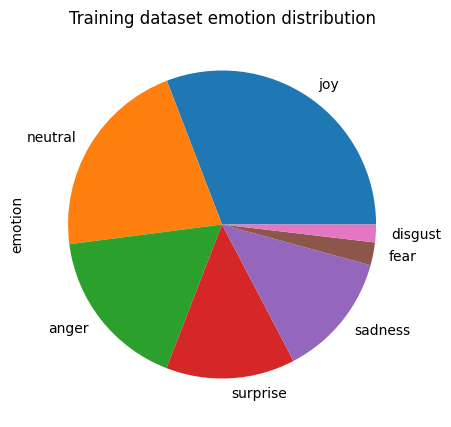
\includegraphics[width=0.6\linewidth]{pieChart.png}
    \caption{Distribuzione delle emozioni}
    \label{fig:dis-emo}
\end{figure}

\bigskip

Di seguito i dati della distribuzione della Figura \ref{fig:dis-emo}:
\begin{lstlisting}
--- Distribution of Emotion ---
joy         0.282908
neutral     0.243030
anger       0.156648
surprise    0.150884
sadness     0.119907
fear        0.025174
disgust     0.021448
\end{lstlisting}

\bigskip

Esempi di dati da predirre. Nella Figura \ref{fig:image1} ci aspettiamo che il modello ritorni \verb|anger| e nella Figura \ref{fig:image2} invece deve tornare \verb|joy|.
\begin{figure}[H]
    \centering
    \begin{subfigure}{0.4\linewidth}
        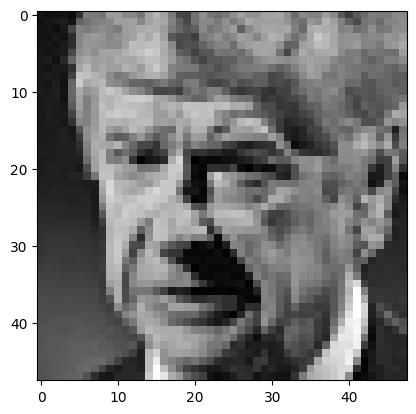
\includegraphics[width=\linewidth]{image.png}
        \caption{Testo associato:\\ unethical human being.}
        \label{fig:image1}
    \end{subfigure}
    \hfill
    \begin{subfigure}{0.4\linewidth}
        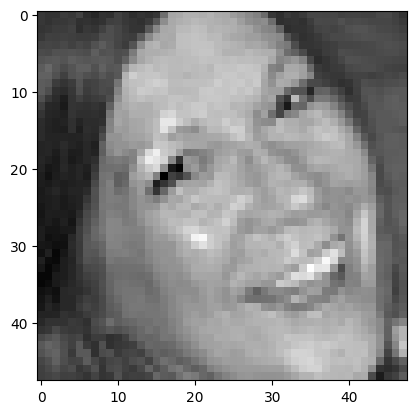
\includegraphics[width=\linewidth]{image2.png}
        \caption{Testo associato:\\ oh my god oh my god congrats!!!}
        \label{fig:image2}
    \end{subfigure}
    \caption{Coppia associata con immagine e frase}
    \label{fig:main}
\end{figure}

\bigskip

Il nostro modello deve ritornare una distribuzione di probabilità, quindi abbiamo associato a ciascuna emozione un numero e ai numeri un vettore. Quindi abbiamo usato una combinazione di \textbf{encoder} e \textbf{categorical encoding} per eseguire questa associazione da emozione a numero a vettore in modo automatico.

\bigskip

\begin{lstlisting}[language=Python, caption=Pre-processing delle frasi]
label_encoder = LabelEncoder()
encoded_emotions = label_encoder.fit_transform(emotions)
categorical_emotions = tf.keras.utils.to_categorical(encoded_emotions, num_classes=len(label_encoder.classes_))

max_words = 20000
tokenizer = Tokenizer(num_words=max_words, oov_token='<OOV>')
tokenizer.fit_on_texts(texts)
text_sequences = tokenizer.texts_to_sequences(texts)
text_padded = pad_sequences(text_sequences, padding='post')
\end{lstlisting}

\bigskip

\begin{table}[!h]
\centering
\begin{tabular}{|c|c|c|}
\hline
Emotion & Number & Vector \\
\hline
Anger & 0 & $\begin{bmatrix} 1 & 0 & 0 & 0 & 0 & 0 & 0 \end{bmatrix}$ \\
Disgust & 1 & $\begin{bmatrix} 0 & 1 & 0 & 0 & 0 & 0 & 0 \end{bmatrix}$ \\
Fear & 2 & $\begin{bmatrix} 0 & 0 & 1 & 0 & 0 & 0 & 0 \end{bmatrix}$ \\
Joy & 3 & $\begin{bmatrix} 0 & 0 & 0 & 1 & 0 & 0 & 0 \end{bmatrix}$ \\
Neutral & 4 & $\begin{bmatrix} 0 & 0 & 0 & 0 & 1 & 0 & 0 \end{bmatrix}$ \\
Sadness & 5 & $\begin{bmatrix} 0 & 0 & 0 & 0 & 0 & 1 & 0 \end{bmatrix}$ \\
Surprise & 6 & $\begin{bmatrix} 0 & 0 & 0 & 0 & 0 & 0 & 1 \end{bmatrix}$ \\
\hline
\end{tabular}
\caption{Emotion Encoding}
\label{tab:emotion_encoding}
\end{table}


Una volta terminato il pre-processing del dataset, esso è stato diviso nelle seguenti porzioni:
\begin{itemize}
    \item Percentuale dati di train: $80\%$
    \item Percentuale dati di validation: $10\%$
    \item Percentuale dati di test: $10\%$
\end{itemize}
Il dataset di immagine, testo e emozione è lungo 25503, quindi avremo circa 20402 dati di train e 2550 dati di validation e test.

\bigskip

Per valutare le performance del nostro modello, abbiamo utilizzato metriche standard come l'\textbf{accuracy} e la \textbf{loss} function. Le emozioni prese in considerazioni sono 7, quindi un modello completamente randomico ha una precisione del $14\%$.

\subsection{Primo modello (EmotionBoost)}
L'obbiettivo del primo modello era quello di vedere se, usando dei semplici layer, si ottiene un predittore migliore di un modello randomico. Quindi, abbiamo utilizzato una serie di layer \textbf{densi} utilizzando alcune funzioni di ottimizzazione e dei \textbf{dropout}.

\bigskip

Inizialmente abbiamo definito due layer di input per il modello: uno per i dati testuali e uno per le immagini. L'input per i dati testuali ha una forma corrispondente alla lunghezza delle frasi preelaborate ($shape=text\_padded.shape[1]$), mentre l'input per le immagini ha una forma di $(48, 48)$, le dimensioni delle immagini.

\bigskip

Per entrambi i tipi di input, abbiamo applicato dei layer densi. Questi layer sono necessari per \textbf{estrarre} le \textbf{caratteristiche} principali dai dati testuali e dalle immagini. Inoltre, nella parte delle immagini, abbiamo applicato un layer \verb|Flatten| per rendere i dati un vettore unico.

\bigskip

Dopo aver concatenato le due parti, abbiamo applicato un layer di dropout con una probabilità del $50\%$. Il dropout è stato utilizzato per \textbf{prevenire} l'\textbf{overfitting} durante l'addestramento del modello, rimuovendo casualmente alcuni neuroni durante ciascuna iterazione dell'addestramento.

\bigskip

\begin{lstlisting}[language=Python, caption=modello con soli layer densi]
# prima parte
text_input = layers.Input(shape=text_padded.shape[1], dtype=tf.int32)
text_dense_layer = layers.Dense(64, activation='relu')(text_input)

# seconda parte
image_input = layers.Input(shape=(48, 48))
image_dense_layer = layers.Dense(64, activation='relu')(image_input)
image_flatten = layers.Flatten()(image_dense_layer)

concatenated = layers.Concatenate()([text_dense_layer, image_flatten])
dropout_layer = layers.Dropout(0.5)(concatenated)
dense_layer = layers.Dense(64, activation='relu')(image_input)
output_layer = layers.Dense(len(label_encoder.classes_), activation='softmax')(dropout_layer)

model = models.Model(inputs=[text_input, image_input], outputs=output_layer)

optimizer = Adam(learning_rate=0.001)
model.compile(optimizer=optimizer, loss='categorical_crossentropy', metrics=['accuracy'])
model.summary()

checkpoint_callback = ModelCheckpoint("best_model.h5", save_best_only=True, monitor="val_accuracy", mode="max")

early_stopping_callback = EarlyStopping(monitor='val_loss', patience=5, restore_best_weights=True)
\end{lstlisting}

Tramite questo semplice modello con $27335$ parametri si raggiunge una precisione circa del $30\%$ (loss: $1.86$) andando quindi a migliorare la precisione di circa $2.3$ volte rispetto a un modello casuale.

\bigskip

\begin{lstlisting}[language=Python, caption=Risultati ottenuti modello lineare]
80/80 [==============================] - 0s 3ms/step - loss: 1.7102 - accuracy: 0.3106 - precision: 0.5093 - recall: 0.0216
Loss: 1.71, Accuracy: 0.31
\end{lstlisting}

\subsection{Secondo modello (EmotionEnhance)}
In questo seconda prova andiamo a cambiare il preprocessing delle immagini andandole a normalizzare per vedere se avrà un impatto sulla rete.
\begin{lstlisting}[language=Python, caption=Normalizzazione delle immagini]
print("Image", images[i])
norm_images = images / 255
print("Normalized image", norm_images[i])

# ricreaiamo il dataset
text_train, text_test_temp, image_train, image_test_temp, emotion_train, emotion_test_temp = train_test_split(
    text_padded, norm_images, categorical_emotions, test_size=0.2, random_state=42)

text_test, text_val, image_test, image_val, emotion_test, emotion_val = train_test_split(
    text_test_temp, image_test_temp, emotion_test_temp, test_size=0.5, random_state=42)
\end{lstlisting}

Normalizzando le immagini abbiamo portato i valori dei pixel delle immagini tra 0 e 1. Questo processo ha contribuito a far \textbf{convergere} più rapidamente i \textbf{modelli} durante l'addestramento, in quanto i dati normalizzati spesso facilitano l'ottimizzazione. 

\begin{lstlisting}[language=Python, caption=differenza immagine normalizzata]
Image [[57 54 54 ... 69 63 56]
 [57 54 57 ... 67 64 59]
 ...
 [63 69 76 ... 50 56 70]
 [62 65 68 ... 57 64 81]]
Normalized image [[0.22352941 0.21176471 0.21176471 ... 0.27058824 0.24705882 0.21960784]
 [0.22352941 0.21176471 0.22352941 ... 0.2627451  0.25098039 0.23137255]
 ...
 [0.24705882 0.27058824 0.29803922 ... 0.19607843 0.21960784 0.2745098 ]
 [0.24313725 0.25490196 0.26666667 ... 0.22352941 0.25098039 0.31764706]]
\end{lstlisting}

Applicando una semplice operazione di normalizzazione raggiungiamo con lo stesso modello una precisione del $45\%$ (loss: $1.47$) migliorando di $3.2$ volte rispetto a un modello casuale.
\begin{lstlisting}[language=Python, caption=Risultati modello normalizzato]
80/80 [==============================] - 0s 2ms/step - loss: 1.4601 - accuracy: 0.4518 - precision_13: 0.6210 - recall_13: 0.2063
Loss: 1.46, Accuracy: 0.45
\end{lstlisting}

\subsection{Terzo modello (EmotionEvolve)}

In questo modello andiamo ad aggiungere dei layer che eseguono operazioni più elaborate sulle due parti di input per migliorare ulteriormente la precisione. Scegliamo un layer \textbf{Embedding} per il testo e dei layer \textbf{convoluzionali} insieme a un layer di \textbf{pooling} per le immagini.\\

I layer di embedding \textbf{mappano} ogni parola del \textbf{testo} in un vettore di numeri reali, dove parole simili sono rappresentate da vettori vicini nello spazio dell'embedding. Questo aiuta il modello a \textbf{catturare} le \textbf{relazioni} semantiche tra le parole e a gestire la dimensionalità del testo in modo più efficiente. 

\bigskip

Per quanto riguarda i layer convoluzionali invece sono necessari per \textbf{estrarre} \textbf{caratteristiche} significative. I filtri convoluzionali sono matrici di pesi che scorrono sull'immagine e ne calcolano le convoluzioni, evidenziando pattern locali come bordi, texture e forme. L'output di questi filtri convoluzionali contiene informazioni sulle \textbf{features} rilevanti presenti nell'immagine. Abbiamo scelto il layer di \textbf{MaxPooling} perché estrapola meglio le caratteristiche delle immagini.
\\
\begin{lstlisting}[language=Python, caption=modello con layer embedding e convoluzionali]
text_input = layers.Input(shape=text_padded.shape[1], dtype=tf.int32)
embedding_layer = layers.Embedding(input_dim=max_words, output_dim=8, input_length=text_padded.shape[1])(text_input)
text_flatten = layers.Flatten()(embedding_layer)

image_input = layers.Input(shape=(48, 48, 1))
conv_layer = layers.Conv2D(32, (3, 3), activation='relu')(image_input)
pooling_layer = layers.MaxPooling2D((2, 2))(conv_layer)
image_flatten = layers.Flatten()(pooling_layer)

concatenated = layers.Concatenate()([text_flatten, image_flatten])
dropout_layer = layers.Dropout(0.5)(concatenated)
output_layer = layers.Dense(len(label_encoder.classes_), activation='softmax')(dropout_layer)

model = models.Model(inputs=[text_input, image_input], outputs=output_layer)
model.compile(optimizer=optimizer, loss='categorical_crossentropy', metrics=['accuracy'])
\end{lstlisting}

Aggiungendo dei layer che vanno ad operare su i due input abbiamo un aumento di circa 9.2 volte dei parametri arrivando a una precisione del 63\% circa (loss: 1.03) che corrisponde a circa 4.6 volte migliore del modello randomico.

\begin{lstlisting}[language=Python, caption=Risultati terzo modello]
80/80 [==============================] - 1s 10ms/step - loss: 0.9787 - accuracy: 0.6604 - precision_14: 0.7538 - recall_14: 0.5608
Loss: 0.98, Accuracy: 0.66
\end{lstlisting}


\subsection{Quarto modello (EmotionFilter)}
In questo modello, vogliamo capire se scritte troppo lunghe o troppo corte vanno a influenzare il risultato. Quindi, abbiamo limitato il dataset applicando due filtri: uno che toglie i dati con la frase più lunga di 20 parole e uno con meno di 5 parole. Controlliamo anche che la distribuzione delle emozioni non sia cambiata di troppo.
\begin{lstlisting}[language=Python, caption=Riduzione parametri tramite filtri]
data = list(filter(lambda x: len(x["text"].split(" ")) < 20, data))
data = list(filter(lambda x: len(x["text"].split(" ")) > 5, data))
\end{lstlisting}

\bigskip

\begin{lstlisting}[language=Python, caption=Distribuzione emozioni]
Numero di dati = 20335
Numero di dati = 16271

--- Distribution of Emotion ---
joy         0.278287
neutral     0.235450
surprise    0.159609
anger       0.155922
sadness     0.123164
fear        0.024891
disgust     0.022678
\end{lstlisting}

Otteniamo così una precisione del $64\%$, praticamente identica alla prova precendente. Quindi la lunghezza delle frasi non ho una ripercussione marcata sul risultato della predizione. Nei prossimi tentativi continueremo quindi ad usare tutto il dataset.
\begin{lstlisting}[language=Python, caption=Risultati quarto modello]
51/51 [==============================] - 0s 9ms/step - loss: 1.1331 - accuracy: 0.5950 - precision_15: 0.7474 - recall_15: 0.4474
Loss: 1.13, Accuracy: 0.59
\end{lstlisting}

\subsection{Quinto modello (EmotionRefine)}
In questo test, cerchiamo di migliorare il preprocessing del testo. Sono state applicate diverse funzioni, in particolare:
\begin{itemize}
    \item La conversione di tutti i testi in minuscolo, standardizzando così la capitalizzazione delle parole.
    \item Rimozione dei caratteri speciali dai testi, come ad esempio i segni di punteggiatura e altri simboli non alfanumerici. In questo modo si dovrebbe semplificare il testo e a concentrarsi sulle parole e sul loro significato.
    \item Conversione delle emoji presenti nei testi in una rappresentazione testuale. Gli emoji vengono trasformati in una forma leggibile dal computer, ad esempio $":)"$ diventa $"smiling\_face\_with\_smiling\_eyes"$. Questo permette al modello di trattare gli emoji come parte del testo.
    \item Dividere le contrazioni presenti nei testi in parole separate. Ad esempio, la contrazione "can't" potrebbe essere divisa in "can" e "not".
\end{itemize}

\begin{lstlisting}[language=Python, caption=Distribuzione emozioni]
def lowerize(data):
  return list(map(lambda x: x.lower(), data))

def remove_special_chars(data):
  return list(map(lambda x: x.replace('|'.join([re.escape(c) for c in list("#%&*/:\^_{|}~")]), ""), data))

def convert_emojis(data):
  return list(map(lambda x: emoji.demojize(x), data))

def split_contractions(data):
  # df_pre.text = df_pre.text.apply(contractions.fix)
  return data

text_processor = TextPreProcessor(normalize= ['money', 'user', 'time', 'date', 'number', 'phone'],
                                  annotate={"elongated", "repeated", 'emphasis', 'censored'},
                                  fix_html=True, tokenizer=SocialTokenizer(lowercase=True).tokenize,
                                  segmenter="twitter", corrector="twitter", unpack_contractions=False,
                                  spell_correct_elong=True, spell_correction=True, fix_text=True,
                                  dicts=[emoticons])

def df_preprocessing(df_pre):
  df_pre = lowerize(df_pre)
  df_pre = convert_emojis(df_pre)
  df_pre = split_contractions(df_pre)
  df_pre = list(map(lambda x: ' '.join(text_processor.pre_process_doc(x)).strip(), df_pre))
  df_pre = remove_special_chars(df_pre)
  return df_pre
\end{lstlisting}

In questo caso il pre-processing non ha portato grandi benefici a riguardo, ottenendo la stessa percentuale di accuracy. Di conseguenza non verrà utilizzato per la prova successiva.
\begin{lstlisting}[language=Python, caption=Risultati modello normalizzazione migliorata]
82/82 [==============================] - 1s 10ms/step - loss: 1.0767 - accuracy: 0.6256 - precision_16: 0.7433 - recall_16: 0.4981
Loss: 1.08, Accuracy: 0.63
\end{lstlisting}


\subsection{Sesto modello (EmotionNorm)}
In questo modello abbiamo aggiunto un layer di normalizzazione sul testo in input. L'obbiettivo era quello di standardizzare il testo per renderlo rilevante quanto le immagini. Invece, per la parte delle immagini abbiamo aggiunto un altro layer convoluzionale e un altro MaxPooling per vedere se eseguiva un'analisi più precisa. 

\begin{lstlisting}
text_input = layers.Input(shape=text_padded.shape[1], dtype=tf.int32)
embedding_layer = layers.Embedding(input_dim=max_words, output_dim=8, input_length=text_padded.shape[1])(text_input)
text_flatten = layers.Flatten()(embedding_layer)
nl = layers.Normalization()(text_flatten)

image_input = layers.Input(shape=(48, 48, 1))
conv_layer = layers.Conv2D(32, (3, 3), activation='relu')(image_input)
pooling_layer1 = layers.MaxPooling2D((2, 2))(conv_layer)
conv_layer2 = layers.Conv2D(24, (3, 3), activation='relu')(pooling_layer1)
pooling_layer2 = layers.MaxPooling2D((2, 2))(conv_layer2)
image_flatten = layers.Flatten()(pooling_layer2)

concatenated = layers.Concatenate()([image_flatten, nl])
dropout_layer = layers.Dropout(0.5)(concatenated)
output_layer = layers.Dense(len(label_encoder.classes_), activation='softmax')(dropout_layer)

model = models.Model(inputs=[text_input, image_input], outputs=output_layer)
model.compile(optimizer=optimizer, loss='categorical_crossentropy', metrics=['accuracy'])
\end{lstlisting}

Il modello ha impiegato più tempo rispetto agli altri per eseguire il training. I parametri sono diminuiti, ma la precisione è salita anche se di poco.

\begin{lstlisting}
80/80 [==============================] - 0s 4ms/step - loss: 0.8812 - accuracy: 0.6922 - precision_4: 0.7824 - recall_4: 0.5808
Loss: 0.88, Accuracy: 0.69
\end{lstlisting}

\subsection{Modello con dataset randomizzato}
Abbiamo sperimentato l'ultimo modello creato andando a modificare il dataset. Il dataset \verb|text_image_emotion_random.csv|, che viene creato con lo script \verb|merge_dataset_randomly.py|, mischia il testo associato all'emozione in modo \textbf{randomico}.

\begin{lstlisting}
113/113 [==============================] - 2s 14ms/step - loss: 1.7825 - accuracy: 0.3734
Loss: 1.78, Accuracy: 0.37
\end{lstlisting}

Il modello ha prodotto chiaramente risultati non soddisfacenti, in particolare una accuracy del $37\%$ e una loss di $1.78$.
Nonostante il testo non combaci con l'immagine, il modello riesce a capire correttamente l'emozione meglio di un modello completamente randomico.

\section{Risultati Sperimentali}
I risultati sperimentali ottenuti dalla valutazione dei modelli proposti per l'emotion detection mostrano un significativo miglioramento delle prestazioni rispetto a un modello casuale. 

\bigskip

Il primo modello, basato su layer densi senza ulteriori elaborazioni, ha raggiunto una accuracy di circa il 31\% e una loss di 1.71. Questo risultato indica un'efficacia superiore rispetto a un modello casuale, con un miglioramento di circa 2.4 volte.

\bigskip

Nel secondo modello, l'introduzione della normalizzazione delle immagini ha portato a un'ulteriore miglioramento delle prestazioni. La accuracy è aumentata al 45\%, con una loss di 1.46. Questo suggerisce che la normalizzazione delle immagini ha contribuito a una migliore convergenza del modello durante l'addestramento.

\bigskip

Al terzo modello, che ha introdotto layer più complessi come l'embedding per il testo e layer convoluzionali per le immagini, ha raggiunto una accuracy del 66\% e una loss di 0.98. Questo rappresenta un significativo miglioramento rispetto ai modelli precedenti, con un'efficacia circa 4.7 volte superiore rispetto a un modello casuale, da notare però l'aumento del tempo di training per singola epoca.

\bigskip

Nel quarto modello sono stati applicati dei filtri sulla lunghezza delle frasi, normalizzandole ad una dimensione ragionevole, ottenendo così nelle frasi dei pesi più uniformi e sono stati abbassati i filtri convoluzionali. Ottenendo sempre una accuracy del 59\% e una loss di 1.13 ma in un tempo notevolmente ridotto.

\bigskip

Nel quinto modello abbiamo migliorato il preprocessing del testo applicando diverse funzioni per il miglioramento del testo da analizzare. Anche in questo caso abbiamo ottenuto una accuracy del 63\% e una loss di 1.08.

\bigskip


Infine, nel sesto e ultimo modello abbiamo aggiunto un layer di normalizzazione sul testo in input. L'obbiettivo era quello di standardizzare il testo per renderlo rilevante quanto le immagini. Invece, per la parte delle immagini abbiamo aggiunto un altro layer convoluzionale e un altro MaxPooling per vedere se faceva un'analisi più precisa. Ottenendo così una accuracy del 69\% e una loss del $0.88$.

\begin{table}[H]
\begin{adjustwidth}{-0.5cm}{}
\centering
\begin{tabular}{@{}llllll@{}}
\toprule
\textbf{Modello} & \textbf{Accuracy} & \textbf{Loss} & \textbf{Parametri} & \textbf{Tempo su epoca} & \textbf{Epoche}  \\ \midrule
1) EmotionBoost & 31\% & 1.71 & 27335 & Circa 4 sec  & 14 \\
2) EmotionEnhance & 45\% & 1.46 & 27335 & Circa 4 sec & 40 \\
3) EmotionEvolve & 66\% & 0.98 & 280727 & Circa 27 sec & 16 \\
4) EmotionFilter & 59\% & 1.13 & 250463 & Circa 14 sec & 13 \\
5) EmotionRefine & 63\% & 1.08 & 253823 & Circa 14 sec & 94 \\
6) EmotionNorm & 69\% & 0.88 & 186512 & Circa 5 sec & 28\\ \bottomrule
\end{tabular}
\caption{Risultati sperimentali dei modelli per l'emotion detection}
\label{tab:results}
\end{adjustwidth}
\end{table}

\subsection{Confronto tra modelli differenti}

Dopo aver sperimentato con diversi metodi i miglioramenti del modello con immagine e testo, lo abbiamo confrontato rispettivamente con modelli di:
\begin{enumerate}
    \item Immagine
    \item Testo
    \item Testo + Immagine
\end{enumerate}

Ottenendo così i seguenti risultati, che riportano il modello con testo e immagine migliore degli altri. Di seguito mostriamo i risultati in tabella:


\begin{table}[H]
\begin{adjustwidth}{-0.5cm}{}
\centering
\begin{tabular}{@{}llllll@{}}
\toprule
\textbf{Modello} & 
\textbf{Accuracy} &
\textbf{Loss} &
\textbf{Parametri} &
\textbf{Precision} &
\textbf{Recall}
\\ \midrule
 Testo & 60\%  & 1.12 & 187167  & 72\% & 40\%  \\
 Immagine & 61\% & 1.06 & 24063 & 76\% & 45\% \\
 Testo + immagine & 69\% & 0.88 & 186512 & 78\% & 58\% \\
\bottomrule
\end{tabular}
\caption{Risultati sperimentali tra modelli differenti}
\label{tab:results}
\end{adjustwidth}
\end{table}


I modelli presi in esame di testo e immagine per la tabella sono i migliori che abbiamo prodotto e sono disponibili nei notebook \verb|image_model.ipynb| e \verb|image_model.ipynb|. La fusione dei due modelli porta quindi ha una miglioria su ogni parametro: in particolare abbiamo un +8\% su accuracy, -0.18 su loss (NB: non è considerato un parametro confrontabile), +2\% su precision e +13\% su recall. I parametri del modello concatenato si allineano a quelli del testo. Abbiamo quindi mostrato che se vengono concatenati due modelli che vogliono estrapolare la stessa feature migliorano tutti i parametri.

\section{Discussione e Conclusioni}
I risultati ottenuti confermano l'efficacia del nostro modello multimodale nel problema dell'emotion detection. Tuttavia, vi sono ancora margini di miglioramento.
Il nostro metodo si è dimostrato valido nel contesto specifico dell'emotion detection, fornendo risultati promettenti. Tuttavia, è importante considerare le limitazioni e i \textbf{bias} presenti nel nostro approccio.
Le principali limitazioni del nostro lavoro potrebbero includere la dimensione del \textbf{dataset} e la \textbf{complessità} computazionale del modello proposto. Inoltre, la maturità tecnologica della soluzione potrebbe essere migliorata attraverso ulteriori sperimentazioni e ottimizzazioni.
Per migliorare il nostro lavoro, si potrebbero esplorare nuove tecniche di \textbf{preprocessing} dei dati, di raccogliere e utilizzare dataset più ampi e diversificati, e di esplorare approcci più avanzati come ad esempio il \textbf{transfer learning}.
\end{document}
